\documentclass[dvipsnames]{beamer}
\usepackage[utf8]{inputenc}
\usepackage[spanish]{babel}
\usepackage{subfigure, wrapfig}
\usepackage{multirow}
\usepackage{graphicx}
\usepackage{tikzsymbols}

\date{} %not show date

%beamer's options
\usetheme{Montpellier}
\author{Gustavo Rivas Gervilla}
\title{Spark \& IoT}

\setbeamertemplate{section in toc shaded}[default][50]
%beamer's colors
\setbeamercolor{section in toc}{fg=orange}
\setbeamercolor{section in toc shaded}{fg=orange}
\setbeamercolor{structure}{fg=brown}
\setbeamercolor{title}{fg=brown}
\setbeamercolor{titlelike}{fg=brown}

\definecolor{deepBlue}{RGB}{10, 9, 68}
\definecolor{deepYellow}{RGB}{219, 219, 8}
\definecolor{deepRed}{RGB}{130, 20, 6}
\definecolor{orangeRed}{RGB}{211, 50, 10}


\begin{document}
	\begin{frame}[plain]
		\titlepage
	\end{frame}
		
	\begin{frame}
		\frametitle{Contenido}
		\tableofcontents
	\end{frame}
	
	\AtBeginSection[]{
		\begin{frame}
			\frametitle{Contenido}
			\tableofcontents[currentsection]
		\end{frame}
	}
	
	\section{Introducción}
	
	\begin{frame}
		\begin{itemize}
			\item ¿Qué es el IoT?
			\item ¿Qué se quiere de este proyecto? $\longrightarrow$ \textcolor{orange}{\textbf{Spark}}
		\end{itemize}		
	\end{frame}

        \begin{frame}
          \begin{itemize}
          \item Muchos dispositivos de diversa naturaleza.
          \item Intercambio y envío de información \textbf{continuo}.
          \item \textcolor{deepRed}{Gran cantidad} de datos de diversa naturaleza $\Rightarrow$ \textcolor{SkyBlue}{\textbf{CC}}. 
          \end{itemize}
        \end{frame}

        \begin{frame}
          \begin{itemize}
          \item En 2020 habrá un cuarto de billón de vehículos conectados [Gartner] $\Rightarrow$ \textbf{muchos datos}.
          \item Analizando estos datos podemos: analizar tráfico de una zona o detectar si un conductor no está en condiciones de conducir.
          \item Se propone \textcolor{orange}{\textbf{Spark}} para analizar todos estos datos.
          \end{itemize}
        \end{frame}

        \begin{frame}
          \begin{itemize}
          \item Proyecto académico.
          \item Analizar y procesar datos de vahículos $\Rightarrow$ Panel de monitorización
          \item En su \href{https://github.com/baghelamit/iot-traffic-monitor}{\textcolor{deepBlue}{GitHub}} tenéis todo el código disponible \Winkey.
          \end{itemize}
        \end{frame}

        \begin{frame}
          \begin{center}
          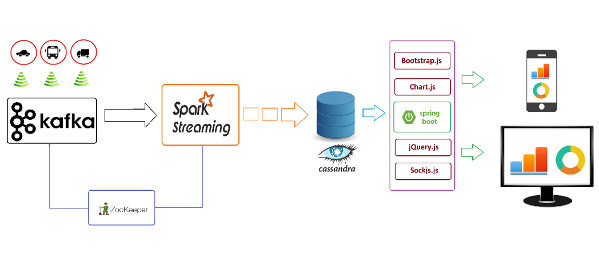
\includegraphics[scale=0.5]{img/arquitectura.jpg}  
          \end{center}          
        \end{frame}

        \section{Kafka: el productor}
	
	\begin{frame}
          \begin{figure}[H]
            \centering
            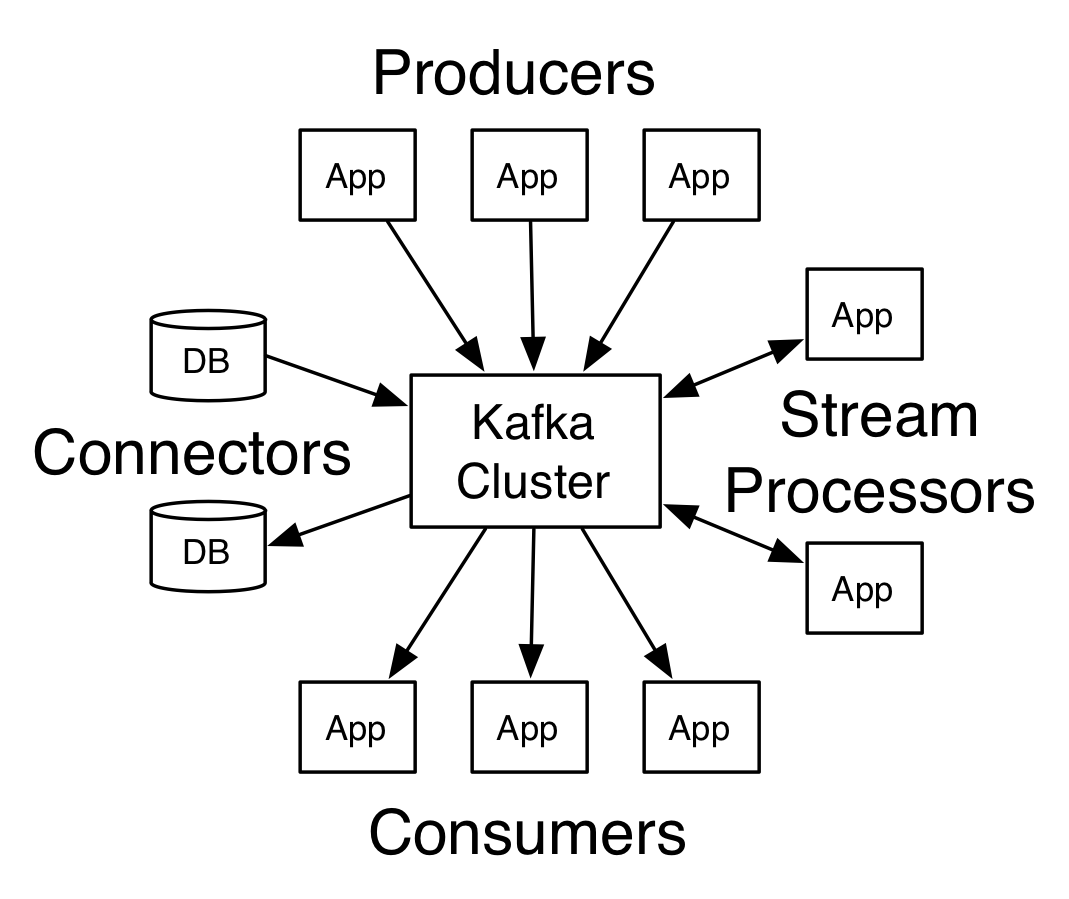
\includegraphics{img/kafka-apis.png}
          \end{figure}
          \begin{itemize}
          \item Sistema de mensajes distribuido.
          \end{itemize}
	\end{frame}

	
	\section{Spark}
	
	\begin{frame}
		¿Qué es Spark?
		\begin{itemize}
			\item Código abierto.
			\item Sistema de propósito general para el procesamiento de Big Data en un sistema cluster.
			\item APIs en: \textcolor{deepBlue}{Python}, \textcolor{deepRed}{Scala} y \textcolor{orangeRed}{Java}.
			\item Con librerías para computación \textbf{paralela}.
		\end{itemize}
	\end{frame}
	
	\section{Spark Streaming}
	
	\begin{frame}
		\begin{itemize}
			\item Librería para computación paralela.
		\end{itemize}
	\end{frame}

        \section{Cassandra}


        \section{Otros casos de interés}


	
	\section{Bibliografía}
	
	\begin{frame}
		\begin{itemize}
		\item \href{https://www.infoq.com/articles/traffic-data-monitoring-iot-kafka-and-spark-streaming}{Art ppal.}
		\end{itemize}
	\end{frame}
	
	\begin{frame}[plain]
		\begin{center}
			\textcolor{orange}{\textbf{¿Preguntas?}}
		\end{center}
	\end{frame}
	
	
\end{document}